\documentclass{article}

% Language setting
% Replace `english' with e.g. `spanish' to change the document language
\usepackage[italian]{babel}
\usepackage{siunitx}
\usepackage{graphicx}
\usepackage{gensymb}
\usepackage{xassoccnt}
\usepackage{setspace}
\usepackage{caption}
\usepackage{hyperref}
\setstretch{1.5}

% Set page size and margins
% Replace `letterpaper' with`a4paper' for UK/EU standard size
\usepackage[letterpaper,top=2cm,bottom=2cm,left=3cm,right=3cm,marginparwidth=1.75cm]{geometry}

% Useful packages
\usepackage{amsmath}
\usepackage{graphicx}
\usepackage[colorlinks=true, allcolors=blue]{hyperref}

\title{
Controllo satellite in orbita intorno alla Terra\\
  \large Progetto Tipologia b - Traccia 2 \\
Controlli Automatici - T

}

\author{A cura di : Giorgio Mastrotucci, Lorenzo Venerandi e Patrick Di Fazio}
\date{}
\begin{document}
\maketitle
\begin{abstract}



\begin{figure}[h!]
\centering
\includegraphics[width=0.3\textwidth]{Schermata 2022-02-04 alle 19.54.38.png}
\caption{\label{fig:orbit}Schema illustrativo della dinamica del satellite}
\end{figure}
\end{abstract}

\begin{center}
\section*{Descrizione del problema}
\end{center}
Il progetto richiede di realizzare un sistema di controllo per un satellite in orbita attorno alla Terra.
Avendo già fornito il primo controllore, le equazioni del sistema risultano:
\[m \Ddot{\rho} = \beta_1\Dot{\rho} + m(k-1)+  (\frac{k_G M}{\rho^{2}} + \rho \omega^{2}) \]
\[\Dot{\omega} = -\frac{2\omega \Dot{\rho} }{\rho} -
\frac{\beta_2 \omega }{m}+ \frac{\tau}{m \rho} ,\]

\noindent
con $\tau(t)$ ingresso libero e velocità angolare $\omega(t)$ misurabile.

\section*{Richieste:}
\begin{enumerate}
\item Riportare il sistema nella forma di stato e linearizzazione.
\item Calcolare la funzione di trasferimento da $\delta U$  a  $\delta Y$,  ovvero la funzione $G(s)$ tale che  \begin{center} $\delta Y (s) = G(s) \delta U (s)$ \end{center}
\item Progettare il regolatore fisicamente realizzabile secondo determinate specifiche.
\item Testare il sistema di controllo linearizzato con :
\[	\omega(t)=8\cdot 10^{-5} \cdot 1(t) \ , \ d(t)= \sum_{k=1}^4 3 \cdot 10^{-5}\cdot sin(0.02 \cdot kt) \ , \  n(t)= \sum_{k=1}^4 3 \cdot 10^{-5}\cdot sin(5\cdot10^{4} \cdot kt)\]
\item Testare il sistema di controllo sul modello non lineare (ed in presenza di $d(t)$ ed $n(t)$).
\end{enumerate}


\begin{center}
\begin{tabular}{||c | c ||} 

 \hline\hline
 $\beta_1$ & $0.3$ \\ 
 \hline
 $\beta_2$ & $0.1$  \\
 \hline
 $m$ & $1$ \\
 \hline
 $m$  & $1.5$  \\
 \hline
 $\rho_e $  & $3\cdot 10^{7}$ \\ [2ex] 
 \hline
\end{tabular}
\end{center}






\section{Sistema in forma di stato e linearizzazione}
\subsection{Forma di stato}
Siano $x_1=\rho$ , $x_2=\Dot{\rho}$ , $x_3=\omega$ stati , $u=\tau$ ingresso e $y=x_3$ uscita del sistema.\\
Riscriviamo le equazioni come sistema in forma di stato\\
\begin{large}
\[
\Dot{x}=
\begin{bmatrix} \Dot{x_1} \\\Dot{x_2} \\ \Dot{x_3}\end{bmatrix} =
\begin{bmatrix} f_1(x,u) \\ f_2(x,u) \\ f_3(x,u)\end{bmatrix} =
\begin{bmatrix} x_2 \\
-\frac{\beta_1 x_2}{m} + (k-1)(\frac{kG M}{x_1^2} - x_1 x_3^2) \\ 
-2\frac{x_3 x_2}{x_1} - \frac{\beta_2 x_3}{m} + \frac{u}{m x_1}  \end{bmatrix}
\]
\[
y=x_3
\]
\end{large}

\subsection{Coppia di equilibrio}
Per rendere il sistema lineare è necessario calcolare i punti di equilibrio $x_e$ e $u_e$.\\
Da specifica sappiamo che $x_{1e}=\rho_e$, quindi poniamo
\begin{large}
\[
\begin{bmatrix} f_1(x_e,u_e) \\ f_2(x_e,u_e) \\ f_3(x_e,u_e)\end{bmatrix} =
\begin{bmatrix} x_{2e} \\
-\frac{\beta_1 x_{2e}}{m} + (k-1)(\frac{kG M}{x_{1e}^2} - x_{1e} x_{3e}^2) \\ 
-2\frac{x_{3e} x_{2e}}{x_{1e}} - \frac{\beta_2 x_{3e}}{m} + \frac{u}{m x_{1e}}  \end{bmatrix} =
\begin{bmatrix} 0 \\ 0 \\ 0\end{bmatrix}
\]
\end{large}
Ricaviamo quindi la coppia di equilibrio:
\begin{large}
\[
x_e=\begin{bmatrix} x_{1e} \\ x_{2e} \\ x_{3e}\end{bmatrix}=
\begin{bmatrix} 3\cdot10^7 \\ 0 \\ 1.215\cdot10^{-4}\end{bmatrix}
\]
\[
u_e=364.63
\]
\end{large}


\subsection{Linearizzazione}
Occorre quindi passare dal modello non linearizzato
\[
\Dot{x}=f(x,u)
\]
\[
y=g(x,u)
\]
\noindent
a quello linearizzato nell'intorno della coppia di equilibrio $(x_e,u_e)$
\[
\delta\Dot{x}=A\delta{x}+B\delta{u}
\]
\[
\delta{y}=C\delta{x}+D\delta{u}
\]
\noindent
Determiniamo quindi le matrici A, B, C, D:
\begin{large}
\[
A=\frac{ \delta{f(x,u)}}{\delta{x}}=
\begin{bmatrix}\frac{\delta{f_1}}{\delta{x_1}} & \frac{\delta{f_1}}{\delta{x_2}}    
& \frac{\delta{f_1}}{\delta{x_3}}\\ 
\frac{\delta{f_2}}{\delta{x_1}} & \frac{\delta{f_2}}{\delta{x_2}}& \frac{\delta{f_2}}{\delta{x_3}} \\
\frac{\delta{f_3}}{\delta{x_1}} & \frac{\delta{f_3}}{\delta{x_2}}& \frac{\delta{f_3}}{\delta{x_3}}
\end{bmatrix}|_{u=u_e}^{x=x_e} = 
\begin{bmatrix}0&1&0\\0&-0.3&-3.646\cdot{10}^3\\0&0&-0.1\\\end{bmatrix}
\]

\[
B=\frac{ \delta{f(x,u)}}{\delta{u}}=
\begin{bmatrix}\frac{\delta{f_1}}{\delta{u}}\\ \frac{\delta{f_2}}{\delta{u}}\\ \frac{\delta{f_3}}{\delta{u}}\end{bmatrix}|_{u=u_e}^{x=x_e}=
\begin{bmatrix}0\\0\\0.3333\cdot10^7\\\end{bmatrix}
\]

\[
C=\frac{ \delta{g(x,u)}}{\delta{x}}=
\begin{bmatrix}\frac{\delta{g}}{\delta{x_1}} & \frac{\delta{g}}{\delta{x_2}}& \frac{\delta{g}}{\delta{x_3}}\end{bmatrix}|_{u=u_e}^{x=x_e}=
\begin{bmatrix}0 & 0 & 1\end{bmatrix}
\]

\[
D=\frac{ \delta{g(x,u)}}{\delta{u}}|_{u=u_e}^{x=x_e}=
\begin{bmatrix}0\end{bmatrix}
\]
\end{large}

\noindent
Sostituendo le matrici nel sistema iniziale otteniamo quindi
\begin{large}
\[
\begin{cases}
\dot{x_1}=x_2\\
\dot{x_2}=-0.3x_2-3.646\cdot10^3 x_3\\
\dot{x_3}=-0.1 x_3+0.3333\cdot10^7 u\\
y=x_3
\end{cases}
\]
\end{large}

\section{Funzione di trasferimento}
Dal sistema linearizzato, passiamo a trovare la funzione di trasferimento: $\delta G(s)$ t.c. $\delta{Y} (s) = G(s)\delta{U} (s)$ e per farlo utilizziamo la trasformata di Laplace.

\begin{large}
\[
\begin{cases}
x(0)=0 \\
G(s)=\frac{\mathcal{L}(y(t))}{\mathcal{L}(u(t))}=\frac{Y(s)}{U(s)}=C(sI-A)^{-1} B +D
\end{cases}
\]
\end{large}
\noindent
Ricaviamo quindi che
\begin{large}
\[
G(s) = 3.3333\cdot 10^{-08}\frac{(s+0.3) (s+7.386\cdot 10^{-08})} {(s+0.3) (s+0.1) (s+2.462\cdot 10^{-08})}
\]
\end{large}



\subsection{Rappresentazione $G(s)$ con diagramma di Bode}

\begin{figure}[!h]
\centering
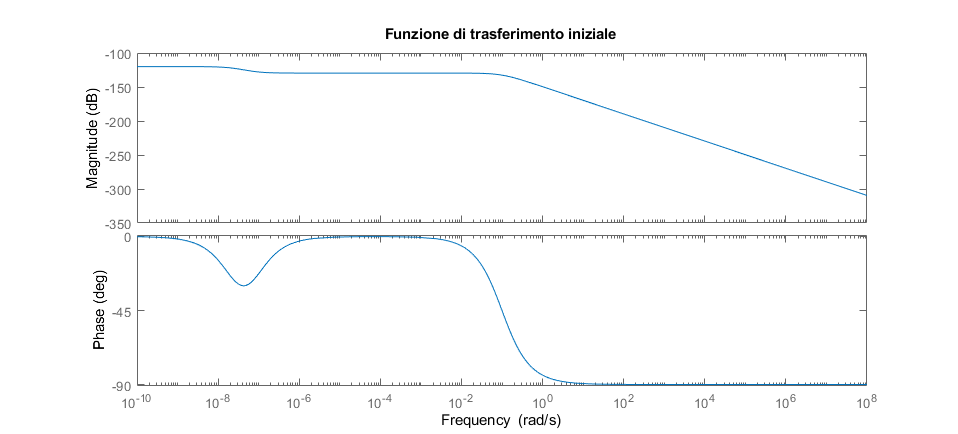
\includegraphics[width=1\textwidth]{grafici/fig1.png}
\caption{\label{fig:bode}Diagramma di Bode di $G(j\omega)$}
\end{figure}
\newpage

\section{Il regolatore}
La funzione di trasferimento in anello aperto è definita come:
\[ L(s) = R(s) \cdot G(s)  \]
verrà ricavata tramite il calcolo di $R(s)$, composto dal regolatore statico $R_s(s)$ e dal regolatore dinamico $R_d(s)$, il regolatore richiesto deve rispettare i vincoli imposti ed essere fisicamente realizzabile.
\subsection{Regolatore Statico}

Dato che $\ G(s)$ non ha un polo nell'origine, per far sì che l'errore a regime sia nullo(1), è necessario inserirne uno. Ponendo il guadagno del regolatore statico a $ \mu_s =\num{e9}$ dB, otteniamo:

\[ R_s = \frac{\mu_s}{s}  \]

\noindent
La funzione di trasferimento estesa al regolatore statico risulta quindi:
\[ G_e(s) = R_s(s) \cdot G(s) \]

\begin{figure}[!h]
\centering
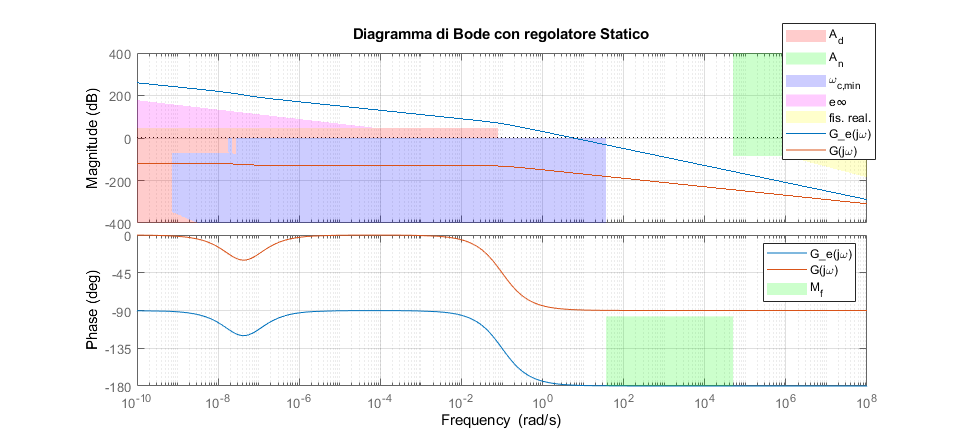
\includegraphics[width=1\textwidth]{grafici/fig2.png}
\caption{\label{fig:orbit}Diagramma di Bode di $G_e(jw)$ con vincoli}
\end{figure}
\noindent
Si nota come non vengano rispettati i vincoli sul tempo di assestamento e sul margine di fase, che verranno fatte rispettare attraverso il regolatore dinamico.


\subsection{Regolatore Dinamico}
 La parte dinamica del regolatore deve rispettare determinate specifiche: il margine di fase $ Mf \geq 40\degree $ (2) per garantire un certo livello di robustezza del sistema regolato. 
La sovraelongazione percentuale massima che il sistema può accettare è $ S \leq 1\% $ (3). Il tempo di assestamento all' $ \epsilon\% = 5\%$ deve essere inferiore a $ T_{a,\epsilon}=0,15s $ (4).\\

\noindent
Per soddisfare queste richieste utilizziamo una rete anticipatrice del tipo
\begin{large}
\[
R_d=\frac{1+\tau s}{1 + \alpha\tau s}
\]
\end{large}

\noindent
È quindi necessario calcolare i parametri $\tau$ ed $\alpha$ utilizzando le formule di inversione
\begin{large}
\[
\tau=\frac{M^*-cos(\varphi^*)}{\omega_c^* sin(\varphi^*)}
\]
\[
\alpha\tau=\frac{cos(\varphi^*)-\frac{1}{M^*}}{\omega_c^* sin(\varphi^*)}
\]
\end{large}

\noindent
nelle quali $M^* > 1$ è l'amplificazione, $\varphi^*$ lo sfasamento e $\omega_c^*$ la frequenza di taglio, cioè la frequenza tale che $|L(j\omega_c^*)|=0$.\\Per rispettare le specifiche è necessario che $\omega_c^*\geq \frac{460}{T^*M_f}$, con $M_f\geq40^{\circ}$ margine di fase, $T^*=0.02 s$ tempo di assestamento e $460$ una costante relativa al tempo di assestamento all'$1\%$.\\
Nel nostro caso (due poli a parte reale negativa) vale $M_f=100\xi$, quindi per ricavare $\xi$ (costante di smorzamento) si utilizza la formula inversa della sovraelongazione percentuale (con $S_\%=1\%$), cioè 
\begin{large}
\[
S_\%=100 e^{\frac{-\pi\xi}{\sqrt{1-\xi^2}}} \longrightarrow \xi\approx 0.83
\]
\end{large}
Ricaviamo quindi $M_f=83^{\circ}$ e $\omega_c^*\geq 36.94 \frac{rad}{s}$, sapendo inoltre che
\begin{large}
\[
M^*=10^{-\frac{|G_e(j\omega_c^*)|_{dB}}{20}}
\varphi
\]
\[
\varphi^*=M_f^*-180-arg\{G_e(j\omega_c^*)\}
\]
\end{large}
possiamo ricavare i parametri $\tau$ ed $\alpha\tau$
\begin{large}
\[
\tau=\frac{M^*-cos(\varphi^*)}{\omega_c^* sin(\varphi^*)}=3.02217
\]
\[
\alpha\tau=\frac{cos(\varphi^*)-\frac{1}{M^*}}{\omega_c^* sin(\varphi^*)}=0.0012
\]
\end{large}
Avendo ricavato la rete anticipatrice riusciamo a calcolare la funzione di trasferimento d'anello aperto:
\begin{large}
\[
L(j\omega)=G_e(s)R_d(s)=\frac{83628 (s+0.3309) (s+0.3) (s+7.386e-08)}{s (s+830.3) (s+0.3) (s+0.1) (s+2.462e-08)}
\]
\end{large}
\begin{figure}[!h]
\centering
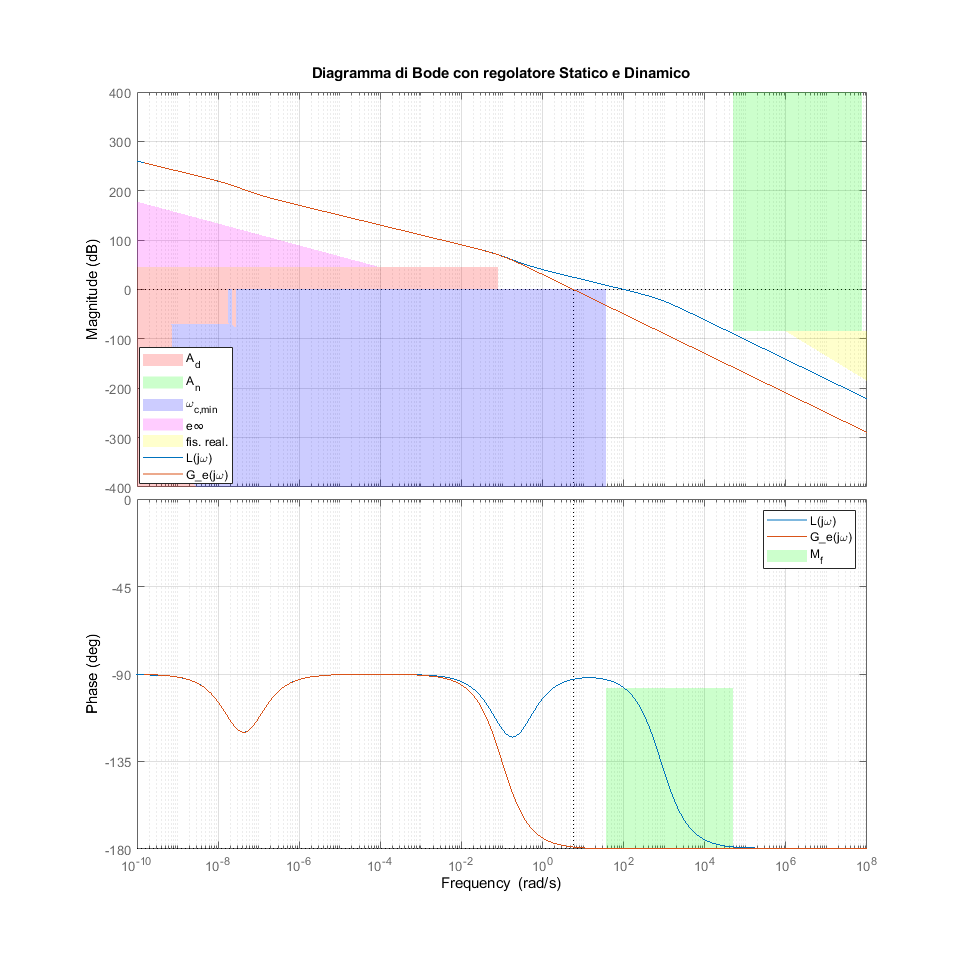
\includegraphics[width=1\textwidth]{grafici/fig3.png}
\caption{\label{fig:orbit}Diagramma di Bode di $L(j\omega)$ con vincoli}
\end{figure}\\
Come si può notare dal grafico soprastante sono stati rispettati tutti i vincoli relativi a tempo di assestamento e margine di fase.
\pagebreak

\section{Test del sistema di controllo sul modello lineare}
\SuspendCounters{subsection}
\subsection{Funzioni di sensitività}
Confrontando questo grafico con la funzione $L(jw)$ rappresentata nella \textit{Figura 4} possiamo controllare la correttezza delle funzioni di sensitività scritte:
\begin{itemize}
\item $S(jw)$ è corretta poiché $|S(jw)| = 1$ per $\omega > \omega c  $ e  $|S(jw)| = \frac{1}{|L(jw)|} $ per $\omega \leq \omega c $
\item $F(jw)$ è corretta poiché $|F(jw)| = 1$ per $\omega \ll \omega c $ e  $|F(jw)| = |L(jw)| $ per $\omega \gg \omega c$
\item $Q(jw)$ è corretta poiché $|Q(jw)| = \frac{1}{|G(jw)|}$ per $\omega \leq \omega c $ e  $|Q(jw)| = |R(jw)| $ per $\omega > \omega c$ (Questo lo si osserva tramite la \textit{Figura 2})

\end{itemize}


\begin{figure}[!h]
\centering
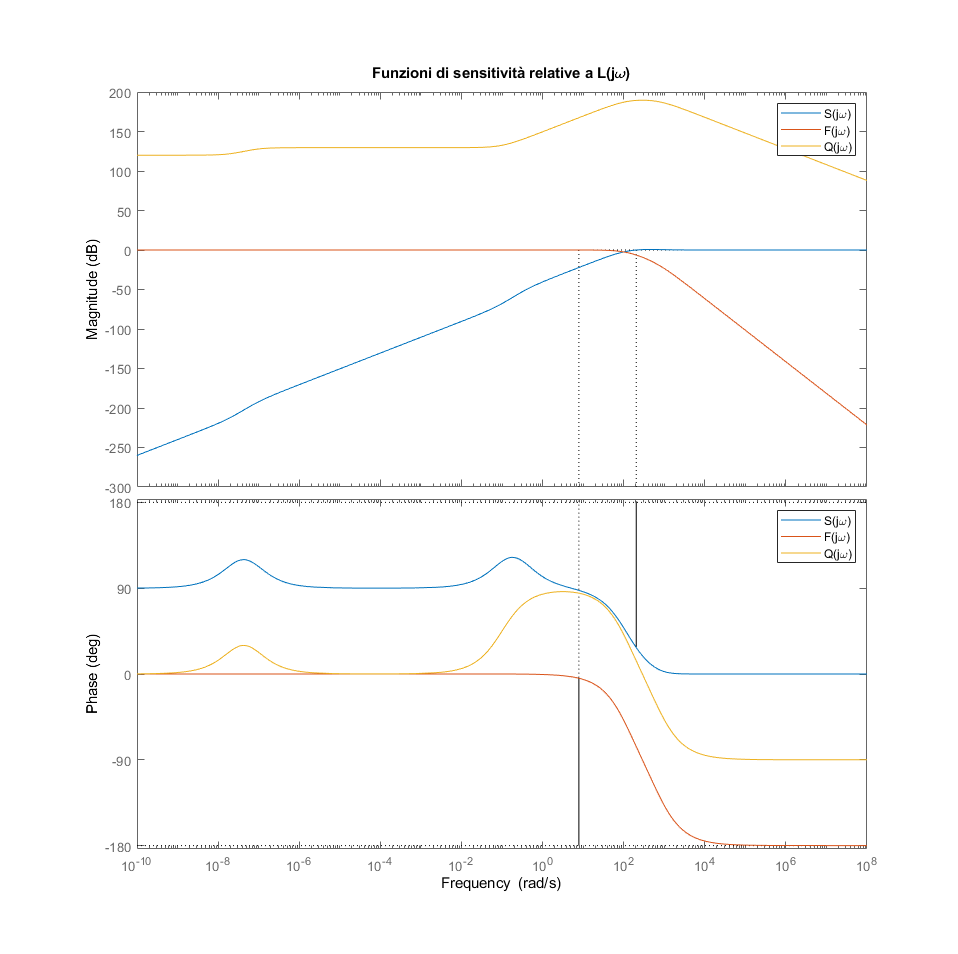
\includegraphics[width=1\textwidth]{grafici/fig10.png}
\end{figure}
\ResumeSuspendedCounters{subsection}


\newpage
\subsection{Risposta al gradino}
Data una funzione gradino $w(t)=8\cdot10{^-5}\cdot1(t)$ la risposta del sistema in anello chiuso rispetta i vincoli del tempo di assestamento e dell'errore a regime, come si può notare dalla figura.

\begin{figure}[!h]
\centering
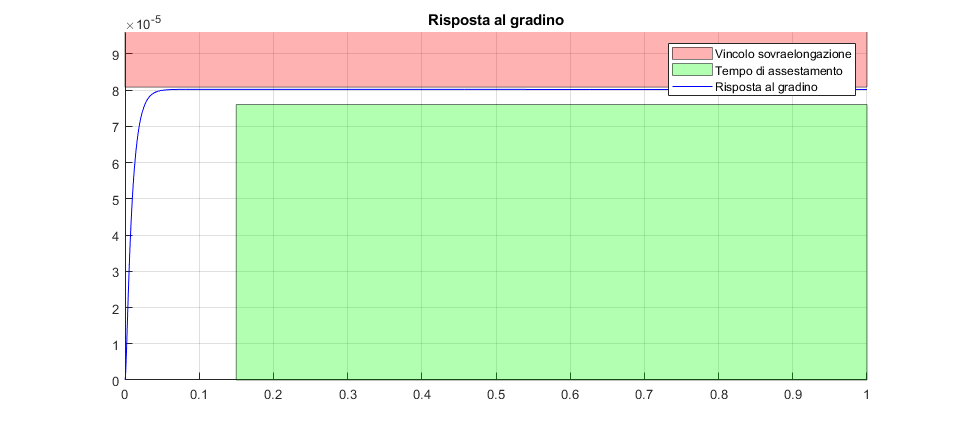
\includegraphics[width=1\textwidth]{grafici/fig4.png}
\caption{\label{fig:orbit}Risposta al gradino $w(t)$}
\end{figure}

\subsection{Disturbo di uscita}
Il sistema riesce inoltre ad attenuare il disturbo di uscita $d(t)=\sum_{k=1}^4 3\cdot10^{-5}\cdot sin(0.02kt)$ quasi completamente (specifica 45 $dB$).
\begin{figure}[!h]
\centering
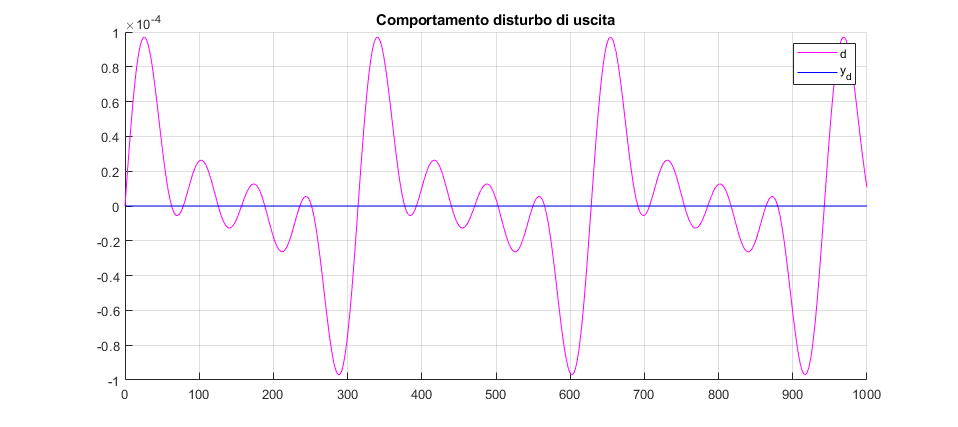
\includegraphics[width=1\textwidth]{grafici/fig5.png}
\caption{\label{fig:orbit}Attenuazione disturbo di uscita $d(t)$}
\end{figure}

\subsection{Disturbo di misura}
Da specifica dobbiamo attenuare il disturbo di misura $n(t)=\sum_{k=1}^4 2\cdot10^{-4}\cdot sin(5\cdot 10^4kt)$. Inizialmente abbiamo generato il grafico con una frequenza di campionamento di 20 $Hz$ e il disturbo risulta poco attenuato, come si nota dal grafico.
\\
\begin{figure}[!h]
\centering
\includegraphics[width=1\textwidth]{grafici/fig7.png}
\caption{\label{fig:orbit}Attenuazione disturbo di uscita $d(t)$}
\end{figure}

\noindent
Aumentando la frequenza di campionamento a 1 $MHz$, più che sufficiente per campionare il segnale 
(\textit{Teorema di Shannon}) otteniamo un grafico che evidenzia come l'attenuazione sia avvenuta e rispetti le specifiche (85 $dB$).

\begin{figure}[!h]
\centering
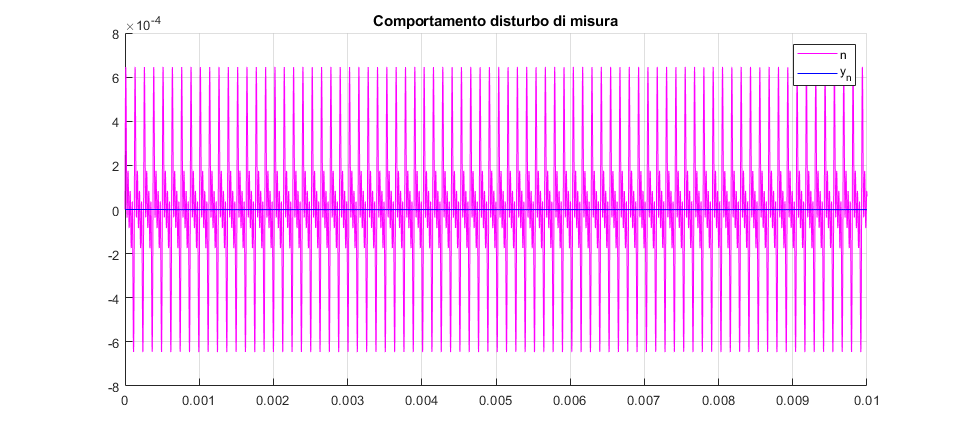
\includegraphics[width=1\textwidth]{grafici/fig6.png}
\caption{\label{fig:orbit}Attenuazione disturbo di uscita $d(t)$}
\end{figure}

\pagebreak


\section{Test del sistema di controllo sul modello non lineare}

\subsection{Sistema non linearizzato su Simulink}
Per lo studio del sistema sul modello non lineare e in presenza di $d(t),n(t)$ abbiamo ricostruito il sistema in anello chiuso

\begin{figure}[!h]
\centering
\includegraphics[width=0.5\textwidth]{schema.png}
\end{figure}

\noindent
in forma non lineare utilizzando Simulink:

\begin{figure}[!h]
\centering
\includegraphics[width=1\textwidth]{grafici/sistema.png}
\caption{\label{fig:orbit}Ricostruzione sistema non lineare}
\end{figure}
\pagebreak
\noindent
Abbiamo inoltre aggiunto l'ingresso in retroazione $y$, il regolatore $R$, i disturbi di uscita $d(t)$ e di misura $n(t)$ e il gradino $w(t)$.
\begin{figure}[!h]
   \begin{minipage}{0.60\textwidth}
     \centering
     \includegraphics[width=1\textwidth]{grafici/misura.png}
   \end{minipage}\hfill
   \begin{minipage}{0.45\textwidth}
     \centering
     \includegraphics[width=1\textwidth]{grafici/uscita.png}
   \end{minipage}
\end{figure}

\newpage 
\subsection{Simulazione sistema non perturbato}

Simulando il sistema rimuovendo i disturbi di misura $n(t)$, di uscita $d(t)$ e l'ingresso a gradino $w(t)$ otteniamo dei grafici degli stati che tendono ai punti di equilibrio, in particolare:
\\

\begin{figure}[!h]
   \begin{minipage}{0.5\textwidth}
     \centering
     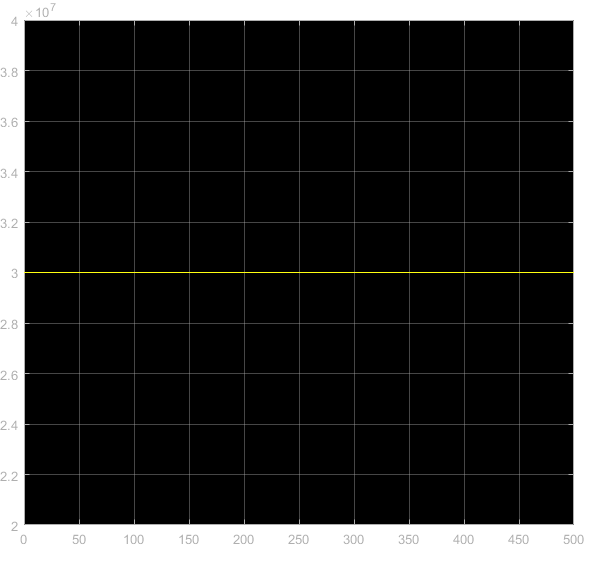
\includegraphics[width=1.03\textwidth]{grafici/x1_1.png}
     \caption*{$x_1\longrightarrow x_{1e}=3\cdot10^7$}
   \end{minipage}\hfill
    \begin{minipage}{0.5\textwidth}
     \centering
     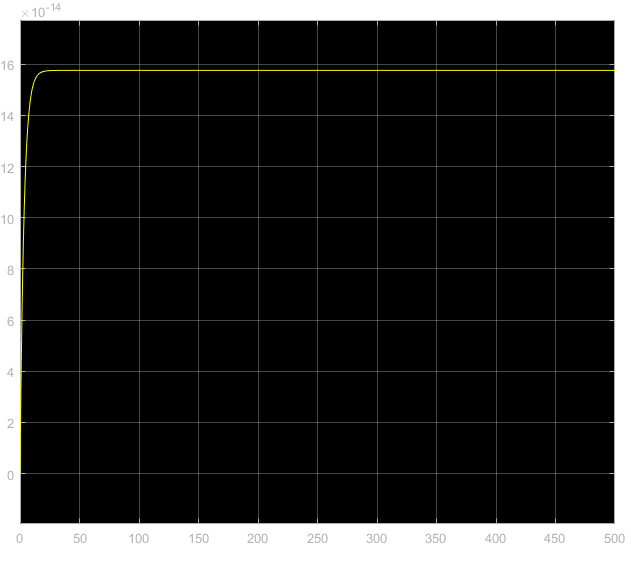
\includegraphics[width=1.1\textwidth]{grafici/x2_1.png}
     \caption*{$x_2\longrightarrow x_{2e}=0$}
   \end{minipage}\hfill
\end{figure}

\begin{figure}[!h]
    \centering
     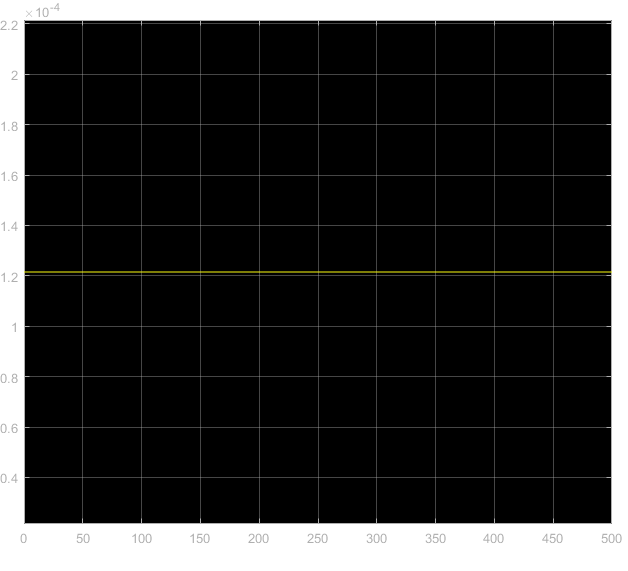
\includegraphics[width=0.7\textwidth]{grafici/x3_1.png}
     \caption*{$y=x_3\longrightarrow x_{3e}=1.215\cdot10^{-4}$}
\end{figure}
\newpage
\noindent
\subsection{Simulazione con disturbi e gradino}
Con l'introduzione dei disturbi si nota un notevole cambiamento nell'andamento dei grafici:
\begin{itemize}
    \item $x_1$ tende a diminuire senza particolari oscillazioni.
    \item $x_2$ ed $x_3$ invece vengono notevolmente perturbati dai disturbi di uscita e misura, ma riescono comunque ad oscillare senza scostarsi dal loro punto di equilibrio.
\end{itemize}

\begin{figure}[!h]
   \begin{minipage}{0.5\textwidth}
     \centering
     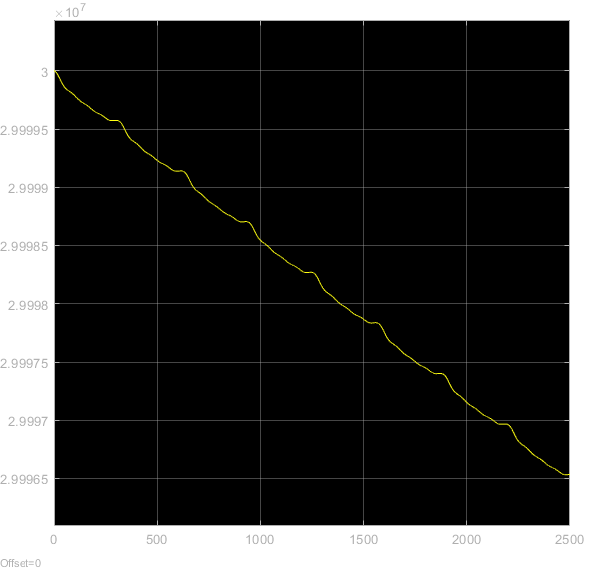
\includegraphics[width=1.06\textwidth]{grafici/x1_2.png}
     \caption*{$x_1$ }
   \end{minipage}\hfill
    \begin{minipage}{0.5\textwidth}
     \centering
     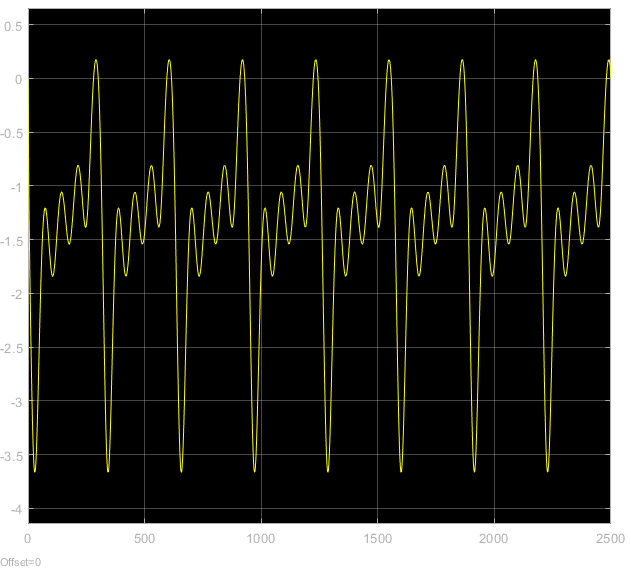
\includegraphics[width=1.1\textwidth]{grafici/x2_2.png}
     \caption*{$x_2$}
   \end{minipage}\hfill
\end{figure}

\begin{figure}[!h]
    \centering
     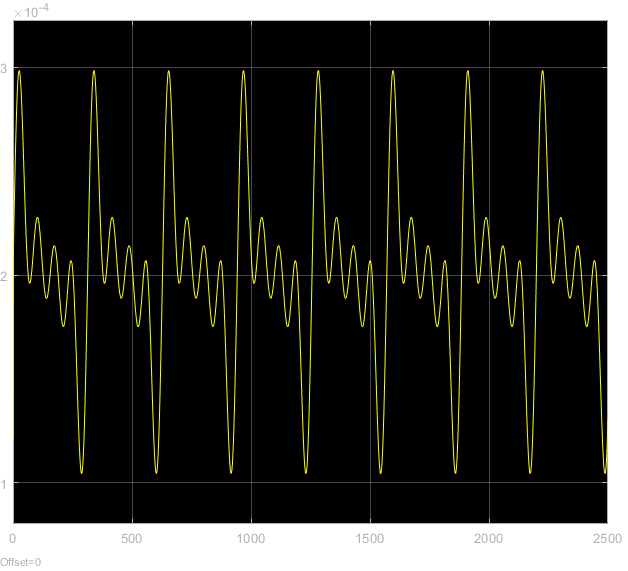
\includegraphics[width=0.6\textwidth]{grafici/x3_2.png}
     \caption*{$y=x_3$}
\end{figure}
\noindent
Simulando per un per un intervallo più lungo abbiamo notato che anche $x_1$ si assesta ad un nuovo punto di equilibrio $\overline{x_{1e}}\simeq1.98955\cdot10^7$, evidenziando la robustezza del sistema anche se soggetto a disturbi.

\begin{figure}[!h]
    \centering
     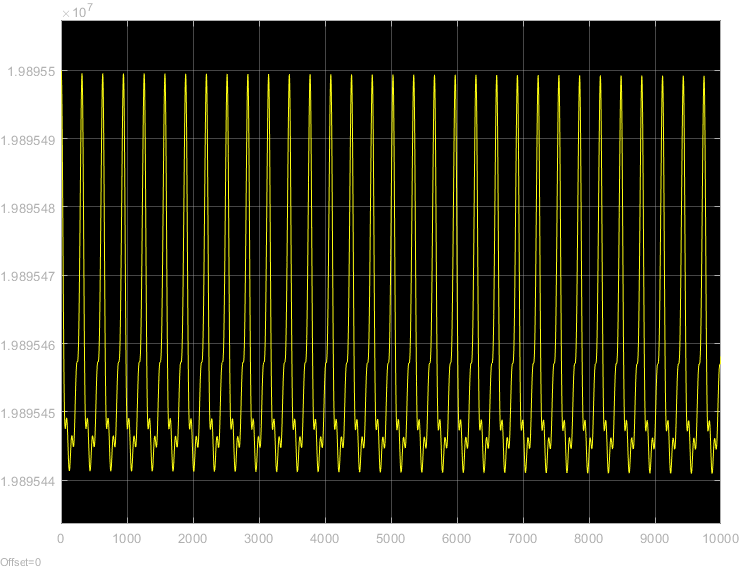
\includegraphics[width=0.6\textwidth]{grafici/x1_1_e.png}
     \caption*{$\overline{x_{1e}}$}
\end{figure}

\subsection{Test con diverse ampiezze di gradino}
\noindent
Nel primo grafico è rappresentata l'uscita in presenza del gradino dato da specifica $W=8\cdot10^{-5}$, si nota come dopo poco tempo (0,05 s) il grafico si sia stabilizzato all'equilibrio.



\begin{figure}[!h]
    \centering
     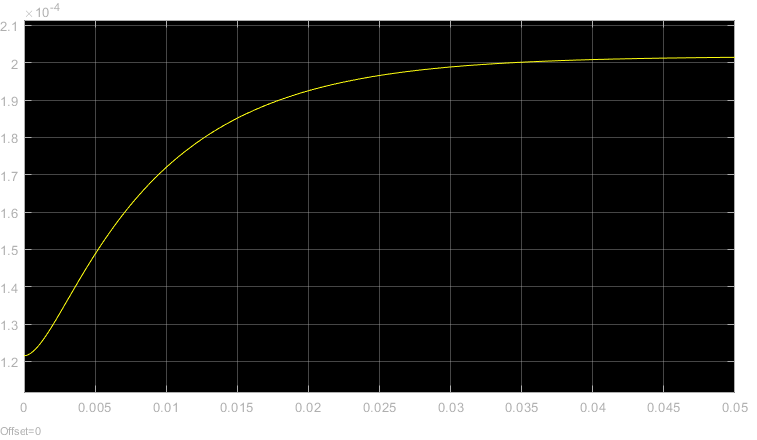
\includegraphics[width=0.75\textwidth]{grafici/gradino_W.png}
     \caption*{$w(t)=W$}
\end{figure}

\noindent
Lo stesso comportamento viene evidenziato dal grafico sottostante, dove abbiamo preso un'ampiezza del gradino di 3 ordini di grandezza superiore ($w(t)=W\cdot4\cdot10^3$), dimostrando la robustezza del sistema anche in seguito a grandi sollecitazioni.

\begin{figure}[!h]
    \centering
     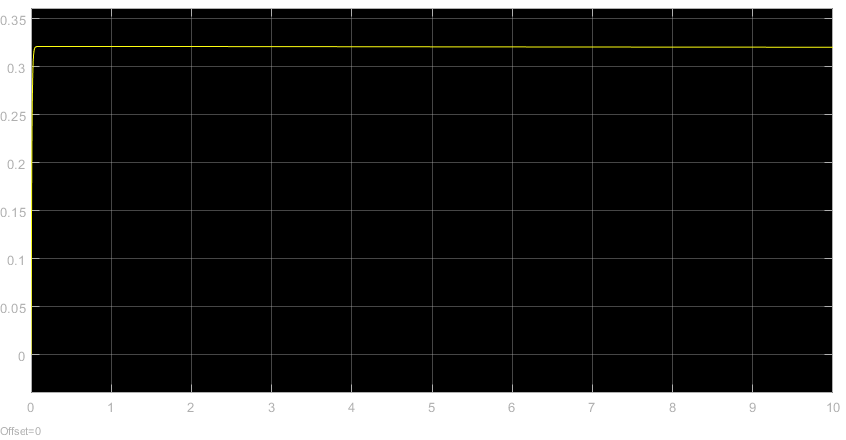
\includegraphics[width=0.75\textwidth]{grafici/grafico_W_4e3.png}
     \caption*{$w(t)=W\cdot4\cdot10^3$}
\end{figure}

\newpage
\noindent
Il comportamento cambia quando l'ampiezza raggiunge valori dell'ordine di $W\cdot10^4$, infatti si notano dei picchi con $\dot{y}\longrightarrow-\infty$, fisicamente impossibili.

\begin{figure}[!h]
    \centering
    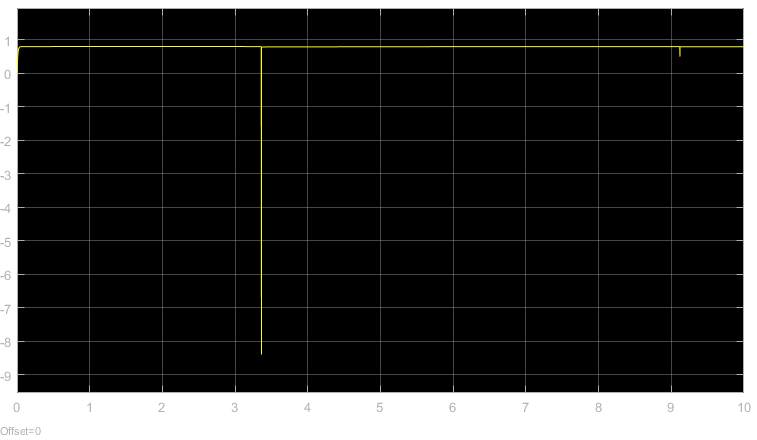
\includegraphics[width=0.75\textwidth]{grafici/grafico_W_1e4.png}
    \caption*{$w(t)=W\cdot10^4$}
\end{figure}

\end{document}